%Matteo Kumar - Leonard Schatt
% Fortgeschrittenes Physikalisches Praktikum
 
\section{Centered Lattices}\label{sec:Q6}
Primitive unit cells of a lattice are the smallest repitition units which can be found and they contain exactly one lattice point per unit cell. However, in some cases they are not able to express the full symmetry of the crystal. Therefore, bigger unit cells can be chosen by centering. Possible lattice structures are body centered with an additional lattice point in the middle of the unit cell (in total two points per unit cell), face centered with additional points on each face of the unit cell (in total four points per unit cell) and basis centered with additional points on the top and bottom face (in total two points per unit cell)~\cite{Schwarzenbach.2001}. One has to keep in mind, that not every crystall structure allows every type of centering. This leads to the 14 Bravais lattices shown in fig.~\ref{fig:bravaisLattices}. When using the centered lattice due to the additional point, destructive interference can additionally occur. Extinction of peaks can be deriven from the structure factor $S$ (see~\ref{sec:Q7}). In general, when considering reflections (h k l), for body centered unit cells reflections with uneven $h+k+l$ vanish, for face centered unit cells just the reflections with either all even or all uneven $h$,$k$,$l$ are visible~\cite{Demtroeder.2016}.

\begin{figure}[ht]
    \centering
    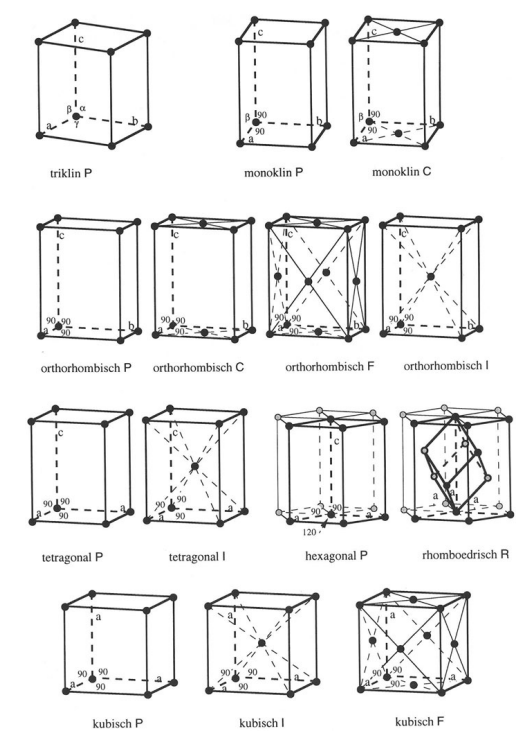
\includegraphics[width = 0.9\linewidth]{Bilder/Grundlagen/lattices.png}
    \caption{The fourteen Bravais lattices are able to describe all crystall structures. They have different degrees of symmetry. For instance, the triclinic lattice has three different lattice vectors and three different angles and therefore just an inversion center, whilst the cubic lattice has a very high degree of symmetry (see also~\ref{sec:Q4}). Figure from~\cite{Schwarzenbach.2001}}
    \label{fig:bravaisLattices}
\end{figure}